\section{Group Operators}

\subsection{Template Convolution}
We can calculate a new image from the original, by applying an \textbf{inverted} template in raster fashion.

\subsubsection{Weighting Coefficients}

Given template $T$, where T is a $3\times 3$ matrix consisting of $9$ weighting coefficients.
\begin{equation} T = 
\begin{bmatrix}
w_{1} & w_{2} & w_{3} \\
w_{4} & w_{5} & w_{6} \\
w_{7} & w_{8} & w_{9}
\end{bmatrix}
\end{equation}

We can calculate a result for the centre pixel of the image we are applying the template to, by calculating the result of the following equation:

\begin{align}
    N_{x,y} = \sum_{i \in template} \sum_{j\in template} w_{i,j} * \mathbf{O}_{x(i),y(j)}
\end{align}

We then have an output image consisting of all the results from each convolution. This is obviously of a smaller size than the original image. This leaves us with three options:

\begin{itemize}
    \itemsep0em
    \item [1] Set the border pixels to black (image usually focused in center)
    \item [2] Assume pixels wrap around 
    \item [3] Reduce template size near edges
\end{itemize}

This leads us to a variety of operators which can be described as a template.

\subsubsection{3x3 Averaging Operator}

The purpose of an averaging operator is to remove noise, and comes with a cost to detail. The template is described as $T_{averaging}$

\begin{equation}
T_{averaging}=
    \begin{bmatrix}
    \frac{1}{9} & \frac{1}{9} & \frac{1}{9} \\
    \frac{1}{9} & \frac{1}{9} & \frac{1}{9} \\
    \frac{1}{9} & \frac{1}{9} & \frac{1}{9}
    \end{bmatrix}
\end{equation}

And we can calculate the new image, setting the border to black, with the following equation:

\begin{equation}
    N_{x,y} = \frac{1}{9} \sum_{i \in 3} \sum_{j \in 3} \mathbf{O}_{x(i),y(j)}
\end{equation}

\subsubsection{Non-symmetric templates}
The template is flipped around on both axes, (inverse template). For deep learning templates this is not necessary as they are usually symmetric.
\\
For a non symmetric template, the convolution is performed as follows:

\begin{align}
    O \times T = \sum_{(x,y)\in W} I_{x,y} T_{x-i,y-j}
\end{align}

\subsubsection{Template Convolution via Fourier Transform}

The convolution theorem allows for fast computation via the FFT (Fast Fourier Transform) for templates $size(T) \geq 7$.

This can be described via:

\begin{align}
    P * T = \mathcal{F}^{-1}(\mathcal{F}(P).\times\mathcal{F}(T)) \\ \\
    \text{Template convolution *} \\
    \text{Fourier transform of the picture }\mathcal{F}(P) \\
    \text{Fourier transform of the template }\mathcal{F}(T) \\
    \text{\textbf{Point by point multiplication for sampled signals }} (.\times)
\end{align}

\subsection{2D Gaussian Function}

The Gaussian function can be used to calculate template values. A commonly used example of this would be Gaussian blur. There is a compromise between the variance and the window size.

\begin{equation}
    g(x,y,\sigma) = \frac{1}{2\pi\sigma^{2}}e^{\frac{-(x^{2}+ y^{2})}{2\sigma^{2}}}
\end{equation}

Given a $\sigma$ value of $1$, we can form a $5\times5$ template which has the following visualisation.

\begin{figure}[ht]
    \centering
    \begin{subfigure}[b]{.5\linewidth}
    \centering
        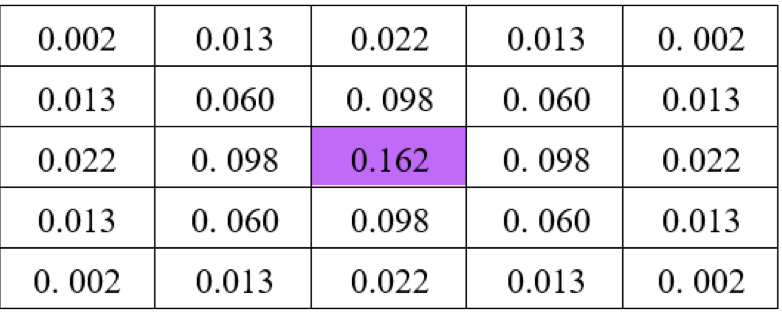
\includegraphics[scale =0.3]{Images/gausstable.png}
    \end{subfigure}%
    \begin{subfigure}[b]{.5\linewidth}
    \centering
        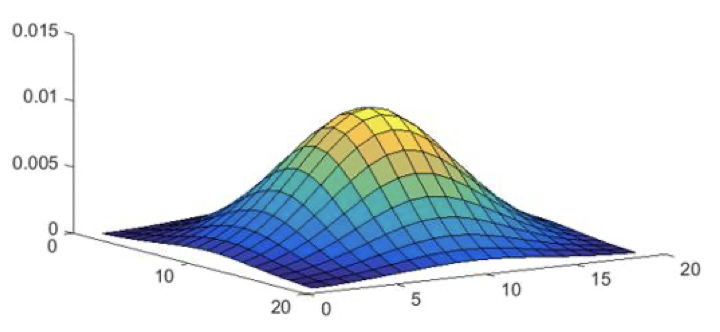
\includegraphics[scale=0.3]{Images/gaussvisual.png}
    \end{subfigure}
    \caption{Visualisation}
    \label{fig:gauss}
\end{figure}

Gaussian averaging is better to a human eye than direct averaging.

\subsection{Median of a Template}

To find the median of a template we can perform the following operation.

\begin{align}
    \text{Original Matrix }\begin{bmatrix}
    2 & 8 & 7 \\
    4 & 0 & 6 \\
    3 & 5 & 7
    \end{bmatrix} \\
    \text{Flattened Vector}
    \begin{bmatrix}
    2 & 8 & 7 & 4 & 0 & 6 & 3 & 5 & 7
    \end{bmatrix} \\
    \text{Sorted Vector}
    \begin{bmatrix}
    0 & 2 & 3 & 4 & \textbf{5} & 6 & 7 & 7 & 8
    \end{bmatrix}
\end{align}

The median is the centre element of a rank ordered set of template points. We preserve the edges and remove salt and pepper noise.

